\documentclass[aspectratio=169,10pt]{beamer}

\usetheme{Madrid}
\usecolortheme{seahorse}

\usepackage{amsmath,amssymb,amsfonts}
\usepackage{mathtools}
\usepackage{xcolor}
\usepackage{listings}
\usepackage{xfrac}
\usepackage{graphicx}
\usepackage{hyperref}

\graphicspath{{figures/}}

% Set up listings for code
\lstset{
    language=Python,
    basicstyle=\ttfamily\scriptsize,
    commentstyle=\color{green!50!black}\itshape,
    keywordstyle=\color{blue}\bfseries,
    stringstyle=\color{red},
    showstringspaces=false,
    breaklines=true,
    frame=single,
    numbers=left,
    numberstyle=\tiny,
    xleftmargin=15pt,
}

% Set footer
\setbeamertemplate{footline}[frame number]

\title{Chapter 26: Resolvents \& Fixed Points}
\subtitle{Zeros of Sums of Monotone Operators}
\author{Convex Analysis and Monotone Operator Theory}
\date{\today}

\begin{document}

% ============================================================================
% TITLE SLIDE
% ============================================================================

\begin{frame}
  \titlepage
  \vspace{-1cm}
  \begin{center}
    \footnotesize
    Source: Convex Analysis and Monotone Operator Theory in Hilbert Spaces \\
     2nd Edition, 2017
  \end{center}
\end{frame}

% ============================================================================
% OVERVIEW
% ============================================================================

\begin{frame}{Chapter Overview}
  \begin{itemize}
    \item \textbf{Problem:} Find zeros of sums of monotone operators
      \[ \text{Find } x \in \mathcal{H} \text{ such that } 0 \in Ax + Bx \]

    \vspace{0.3cm}
    \item \textbf{Key Concept:} Resolvents and Fixed Points
      \begin{itemize}
        \item Resolvent: $J_A = (\text{Id} + A)^{-1}$
        \item Fixed point: $x = J_A(x) \Leftrightarrow 0 \in Ax$
      \end{itemize}

    \vspace{0.3cm}
    \item \textbf{Main Topics:}
      \begin{enumerate}
        \item Duality and Characterizations
        \item Spingarn's Method of Partial Inverses
        \item Douglas-Rachford Splitting Algorithm
        \item Forward-Backward Splitting
        \item Variational Inequalities
      \end{enumerate}

    \vspace{0.3cm}
    \item \textbf{Applications:} Optimization, proximal methods, splitting algorithms
  \end{itemize}
\end{frame}

% ============================================================================
% SECTION 1: DUALITY AND CHARACTERIZATIONS
% ============================================================================

\section{Duality and Characterizations}

\begin{frame}{Zeros of Sums: Basic Characterizations}

\textbf{Setup:} $A, B: \mathcal{H} \to 2^{\mathcal{H}}$ are operators, $\gamma \in \mathbb{R}_{++}$

\vspace{0.2cm}
Let $\mathcal{P} = \text{zer}(A + B)$ (solutions to $0 \in Ax + Bx$)

\vspace{0.2cm}
Let $\mathcal{Q} = \text{zer}(-A^{-1}(-\text{Id}) - B^{-1})$ (dual problem)

\vspace{0.3cm}
\textbf{Proposition 26.1:} The following characterizations hold:

\begin{enumerate}
  \item[(i)] \textbf{Direct form:}
    \begin{align*}
      \mathcal{P} &= \{x \in \mathcal{H} \mid (\exists u \in \mathcal{Q}) \: -u \in Ax \text{ and } u \in Bx\} \\
      \mathcal{Q} &= \{u \in \mathcal{H} \mid (\exists x \in \mathcal{P}) \: x \in A^{-1}(-u) \text{ and } x \in B^{-1}u\}
    \end{align*}

  \item[(ii)] \textbf{With closed affine subspace:} If $C$ is closed affine and $A = N_C$:
    \[ \mathcal{P} = \{x \in C \mid V^{\perp} \cap Bx \neq \emptyset\}, \quad
       \mathcal{Q} = \{u \in V^{\perp} \mid C \cap B^{-1}u \neq \emptyset\} \]

  \item[(iii)] \textbf{Douglas-Rachford operator:} Let $T_{A,B} = J_A R_B + \text{Id} - J_B$
    \[ \mathcal{P} = J_{\gamma B}(\text{Fix } R_{\gamma A}R_{\gamma B}), \quad
       \mathcal{Q} = ^{\infty}B(\text{Fix } T_{\gamma A,\gamma B}) \]
\end{enumerate}

\end{frame}

\begin{frame}{Douglas-Rachford Splitting Operator}

\textbf{Definition:} For maximally monotone $A, B$, the \textbf{Douglas-Rachford splitting operator} is:
\[ T_{A,B} = J_A R_B + \text{Id} - J_B \]

where:
\begin{itemize}
  \item $J_A = (\text{Id} + A)^{-1}$ is the resolvent
  \item $R_A = 2J_A - \text{Id}$ is the reflected resolvent
\end{itemize}

\vspace{0.3cm}
\textbf{Key Properties (Proposition 26.1(iii)):}

\begin{enumerate}
  \item[(a)] $T_{A,\gamma B}$ is firmly nonexpansive

  \item[(b)] $\mathcal{P} = J_{\gamma B}(\text{Fix } R_{\gamma A}R_{\gamma B}) = J_{\gamma B}(\text{Fix } T_{\gamma A,\gamma B})$

  \item[(c)] $\mathcal{Q} = ^{\infty}B(\text{Fix } R_{\gamma A}R_{\gamma B}) = ^{\infty}B(\text{Fix } T_{\gamma A,\gamma B})$

  \item[(d)] $\mathcal{P} \neq \emptyset \Leftrightarrow \mathcal{Q} \neq \emptyset \Leftrightarrow \text{Fix } T_{\gamma A,\gamma B} \neq \emptyset$
\end{enumerate}

\end{frame}

\begin{frame}{Special Cases}

\textbf{Proposition 26.1(iv):} Suppose $A$ is maximally monotone and $B: \mathcal{H} \to \mathcal{H}$.
Set $T_{A,B} = J_A \circ (\text{Id} - B)$.

Then:
\begin{enumerate}
  \item[(a)] $\mathcal{P} = \text{Fix } T_{\gamma A,\gamma B}$

  \item[(b)] $\mathcal{Q} = B(\mathcal{P})$

  \item[(c)] $\mathcal{P} \neq \emptyset \Leftrightarrow \mathcal{Q} \neq \emptyset \Leftrightarrow \text{Fix } T_{\gamma A,\gamma B} \neq \emptyset$
\end{enumerate}

\vspace{0.3cm}
\textbf{Proposition 26.1(v):} Suppose $A$ is maximally monotone and $B^{-1}: \mathcal{H} \to \mathcal{H}$.
Then:
\[ \mathcal{Q} = \text{Fix}(-\gamma A \circ (B^{-1} - \gamma \text{Id})), \quad \mathcal{P} = B^{-1}(\mathcal{Q}) \]

\vspace{0.3cm}
\textbf{Corollary 26.3:} For maximally monotone $A$ and $\gamma \in \mathbb{R}_{++}$:
\[ \text{Fix } J_A \circ (\text{Id} + \gamma(B - \text{Id})) = \text{Fix } J_{\gamma^{-1}A} \circ B \]

\end{frame}

\begin{frame}{Finite Sums of Operators}

\textbf{Proposition 26.4:} For a finite collection of maximally monotone operators $(A_i)_{i \in I}$, define:
\[ \mathcal{H} = \bigoplus_{i \in I} \mathcal{H}, \quad D = \{(x, \ldots, x) \in \mathcal{H} \mid x \in \mathcal{H}\} \]
\[ \mathcal{J}: \mathcal{H} \to \mathcal{D}, \quad x \mapsto (x, \ldots, x), \quad
   \mathcal{A}: \mathcal{H} \to 2^{\mathcal{H}}, \quad (x_i)_{i \in I} \mapsto \prod_{i \in I} A_i x_i \]

Then for $x = (x_i)_{i \in I} \in \mathcal{H}$:
\begin{enumerate}
  \item[(i)] $D^{\perp} = \{u \in \mathcal{H} \mid \sum_{i \in I} u_i = 0\}$

  \item[(ii)] $N_D x = \begin{cases} \{u \in \mathcal{H} \mid \sum_{i \in I} u_i = 0\} & \text{if } x \in D \\ \emptyset & \text{otherwise} \end{cases}$

  \item[(iii)] $P_D x = \mathcal{J}((1/m)\sum_{i \in I} x_i)$

  \item[(iv)] $P_{D^{\perp}} x = (x_i - (1/m)\sum_{j \in I} x_j)_{i \in I}$
\end{enumerate}

\end{frame}

\begin{frame}[allowframebreaks]{Zeros of Finite Sums}

\textbf{Theorem 26.5:} Suppose $(A_i)_{i \in I}$ are maximally monotone operators where $I = \{1, \ldots, m\}$ with $m \geq 2$.

Then there exists $x \in \text{zer } \sum_{i \in I} A_i$ such that:
\begin{enumerate}
  \item[(i)] $x = x_1 = \cdots = x_m$

  \item[(ii)] $\sum_{i \in I} u_i = 0$

  \item[(iii)] $(\forall i \in I) \quad (x, u_i) \in \text{gra } A_i$

  \item[(iv)] $\sum_{i \in I} \langle x_i, n | u_{i,n} \rangle \to \langle x \mid \sum_{i \in I} u_i \rangle = 0$
\end{enumerate}

\textbf{Proof sketch:}
\begin{itemize}
  \item Define $\mathcal{H}, \mathcal{D}, \mathcal{J}, \mathcal{A}$ as in Proposition 26.4
  \item Note that $(\mathbf{x}_n, \mathbf{u}_n)_{n \in \mathbb{N}}$ lies in $\text{gra } \mathcal{A}$
  \item Convergence follows from Proposition 23.18 and proximal-point iterations
\end{itemize}

\end{frame}

% ============================================================================
% SECTION 2: SPINGARN'S METHOD
% ============================================================================

\section{Spingarn's Method of Partial Inverses}

\begin{frame}{Problem Setup}

\textbf{Spingarn's Method:} A technique for solving constrained monotone operator problems.

\vspace{0.3cm}
\textbf{Problem:} Given:
\begin{itemize}
  \item $A: \mathcal{H} \to 2^{\mathcal{H}}$ is maximally monotone
  \item $V$ is a closed linear subspace of $\mathcal{H}$
  \item The problem $\text{find } x \in V, u \in V^{\perp} \text{ such that } u \in Ax$ has at least one solution
\end{itemize}

\textbf{Goal:} Find $(x^*, u^*) \in V \times V^{\perp}$ such that $u^* \in Ax^*$

\vspace{0.3cm}
\textbf{Application:} Decompose a complex operator problem into subproblems that may be easier to solve.

\vspace{0.3cm}
\textbf{Key decomposition:} $\mathcal{H} = V \oplus V^{\perp}$

\end{frame}

\begin{frame}{Spingarn's Algorithm}

\textbf{Theorem 26.9 (Spingarn):} Let $A: \mathcal{H} \to 2^{\mathcal{H}}$ be maximally monotone, $V$ a closed subspace, and suppose the problem $\text{find } x \in V, u \in V^{\perp}$ such that $u \in Ax$ has at least one solution.

\vspace{0.2cm}
Given $x_0 \in V$, $u_0 \in V^{\perp}$, set for $n = 0, 1, \ldots$:

\begin{align*}
  y_n &= J_A(x_n + u_n) \\
  v_n &= x_n + u_n - y_n \\
  (x_{n+1}, u_{n+1}) &= (P_V y_n, P_{V^{\perp}} v_n)
\end{align*}

\textbf{Then:} There exists a solution $(x, u)$ to the constrained problem such that $x_n \to x$ and $u_n \to u$.

\vspace{0.3cm}
\textbf{Proof idea:}
\begin{itemize}
  \item Decompose $z_n = x_n + u_n$ where $z_n \in \mathcal{H}$
  \item Use proximal-point iterations: $z_{n+1} = J_A z_n$
  \item Project back to $V \times V^{\perp}$ at each step
  \item Convergence follows from Proposition 23.30(ii)
\end{itemize}

\end{frame}

\begin{frame}{Geometric Interpretation}

\begin{center}
  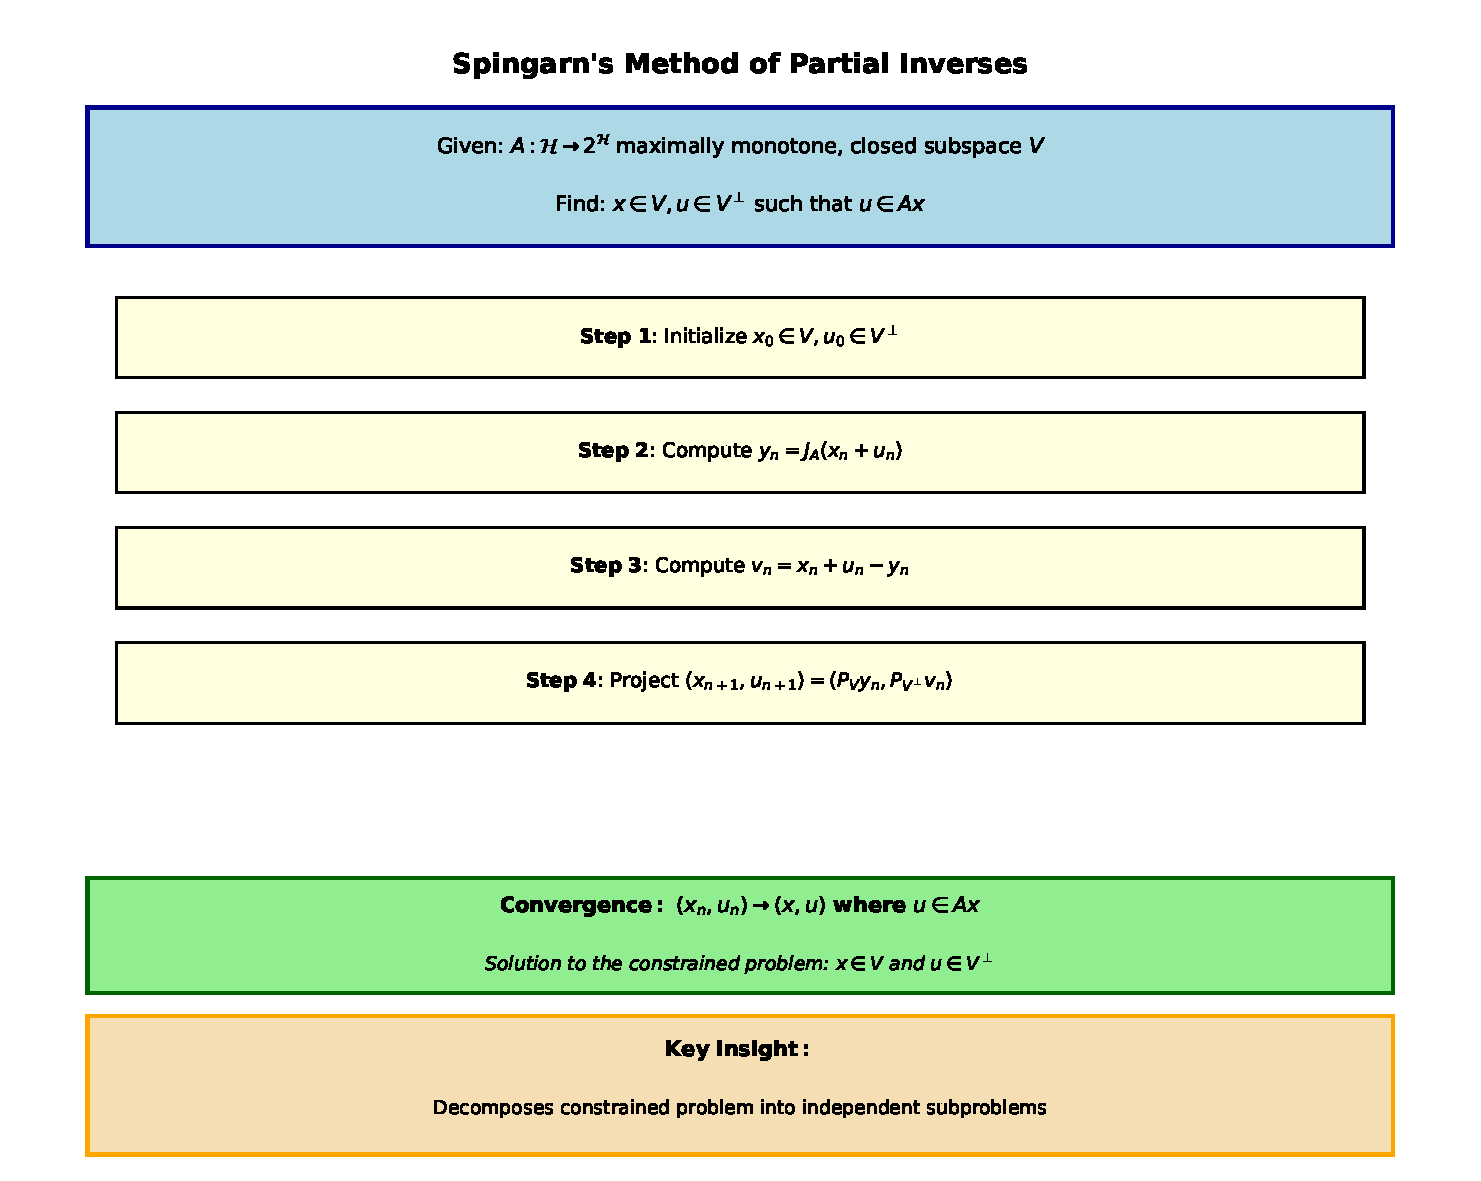
\includegraphics[width=0.9\textwidth]{spingarn_method.pdf}
\end{center}

\textbf{Key insights:}
\begin{itemize}
  \item The algorithm alternates between:
    \begin{enumerate}
      \item Applying the resolvent $J_A$ in full space
      \item Projecting onto the constrained subspaces $V$ and $V^{\perp}$
    \end{enumerate}

  \item The decomposition $\mathcal{H} = V \oplus V^{\perp}$ allows independent handling of components

  \item Solution inherently satisfies $x^* \in V$ and $u^* \in V^{\perp}$
\end{itemize}

\end{frame}

% ============================================================================
% SECTION 3: DOUGLAS-RACHFORD SPLITTING
% ============================================================================

\section{Douglas-Rachford Splitting Algorithm}

\begin{frame}{Standard Splitting Problem}

\textbf{Problem:} Solve the monotone inclusion:
\[ 0 \in Ax + Bx \]

where $A, B: \mathcal{H} \to 2^{\mathcal{H}}$ are maximally monotone operators.

\vspace{0.3cm}
\textbf{Motivation:}
\begin{itemize}
  \item Direct methods may be hard to apply when $A$ or $B$ has no closed form
  \item \textbf{Splitting:} Apply resolvents of $A$ and $B$ separately
  \item Benefits: Each $J_A$ and $J_B$ may be easier to compute individually
\end{itemize}

\vspace{0.3cm}
\textbf{Douglas-Rachford Splitting Algorithm:}

\begin{align*}
  y_n &= J_A(x_n) \\
  x_{n+1} &= x_n + J_B(2y_n - x_n) - y_n
\end{align*}

Equivalently: $x_{n+1} = T_{A,B}(x_n)$ where $T_{A,B} = J_A R_B + \text{Id} - J_B$

\vspace{0.3cm}
\textbf{Fixed point:} $x^* = T_{A,B}(x^*) \Rightarrow x^* \in \text{zer}(A + B)$

\end{frame}

\begin{frame}{Convergence of Douglas-Rachford}

\textbf{Theorem 26.10:} Suppose:
\begin{enumerate}
  \item[(i)] $D$ is a nonempty closed subset of $\mathcal{H}$
  \item[(ii)] $A: \mathcal{H} \to 2^{\mathcal{H}}$ is maximally monotone with $\text{dom } A \subseteq D$
  \item[(iii)] $B: \mathcal{H} \to 2^{\mathcal{H}}$ is maximally monotone
  \item[(iv)] $\text{zer}(A + B) \cap D \neq \emptyset$
\end{enumerate}

Given $x_0 \in D$, set:
\begin{align*}
  y_n &= J_A(x_n) \\
  x_{n+1} &= x_n + J_B(2y_n - x_n) - y_n
\end{align*}

\textbf{Then:} $(x_n)_{n \in \mathbb{N}} \to x^*$ for some $x^* \in \text{zer}(A + B) \cap D$.

\vspace{0.3cm}
\textbf{Proof sketch:}
\begin{itemize}
  \item Show $x_n$ lies in bounded sequence (bounded domain)
  \item Use weak sequential compactness
  \item Apply monotonicity arguments to identify limit point
\end{itemize}

\end{frame}

\begin{frame}[fragile]{Douglas-Rachford Example}

\textbf{Numerical example:} Solve $0 \in \partial f(x) + Bx$ where:
\begin{itemize}
  \item $f(x) = \|x\|_1$ (sparsity-inducing)
  \item $B$ is a linear operator
\end{itemize}

\vspace{0.2cm}
\lstset{basicstyle=\ttfamily\footnotesize}
\begin{lstlisting}
import numpy as np
from scipy.optimize import minimize

# Problem: min ||x||_1 + 0.5 * ||x - b||^2
def soft_threshold(x, lam):
    """Proximal operator of ||.||_1"""
    return np.sign(x) * np.maximum(np.abs(x) - lam, 0)

def douglas_rachford(b, gamma=0.1, n_iter=100):
    """Douglas-Rachford for ||x||_1 + 0.5||x-b||^2"""
    x = np.zeros_like(b)
    for n in range(n_iter):
        # Prox of ||.||_1
        y = soft_threshold(x, gamma)
        # Prox of 0.5||x-b||^2: (I + gamma*(-I)^{-1})^{-1}
        z = (x + gamma * b) / (1 + gamma)
        x = x + z - y
    return x

b = np.array([1.5, -0.5, 0.8])
x_opt = douglas_rachford(b)
print(f"Solution: {x_opt}")
\end{lstlisting}

\end{frame}

\begin{frame}{Convergence Rates}

\textbf{Proposition 26.16 (Linear Convergence):} Let:
\begin{enumerate}
  \item[(i)] $A$ be $\alpha$-strongly monotone, $B$ be $\delta$-cocoercive, $\gamma \in ]0, 2\delta[$

  \item[(ii)] OR $\alpha \leq \beta$, $B$ be $\alpha$-strongly monotone and $\beta$-Lipschitz continuous, $\gamma \in ]0, 2\alpha/\beta^2[$
\end{enumerate}

Let $x_0 \in D$ and set:
\begin{align*}
  y_n &= x_n - \gamma B x_n \\
  x_{n+1} &= J_{\gamma A}(y_n)
\end{align*}

\textbf{Then:} $(x_n)_{n \in \mathbb{N}}$ converges linearly to the unique point in $\text{zer}(A + B)$.

\vspace{0.3cm}
\textbf{Key rates:}
\begin{itemize}
  \item Linear: $\|x_{n+1} - x^*\| \leq \rho \|x_n - x^*\|$ with $\rho < 1$
  \item Rate depends on strong convexity/cocoercivity constants
\end{itemize}

\end{frame}

\begin{frame}[allowframebreaks]{Forward-Backward Algorithm}

\textbf{Problem:} Solve $0 \in Ax + Bx$ where:
\begin{itemize}
  \item $A: \mathcal{H} \to 2^{\mathcal{H}}$ is maximally monotone
  \item $B: \mathcal{H} \to \mathcal{H}$ is single-valued (e.g., differentiable operator)
\end{itemize}

\vspace{0.3cm}
\textbf{Advantage:} Can handle composite inclusion problems directly.

\vspace{0.3cm}
\textbf{Forward-Backward Algorithm:}

\begin{align*}
  y_n &= x_n - \gamma B x_n \quad (\text{forward step on } B) \\
  x_{n+1} &= J_{\gamma A}(y_n) \quad (\text{backward step on } A)
\end{align*}

\vspace{0.3cm}
\textbf{Proposition 26.20:} Suppose $B$ is monotone and $\text{zer}(A + B) \neq \emptyset$, $\gamma \in ]0, \infty[$. Then:
\begin{enumerate}
  \item[(i)] $(x_n)_{n \in \mathbb{N}}$ converges weakly to a solution
  \item[(ii)] If additionally $A$ or $B$ is strictly monotone, convergence is strong
\end{enumerate}

\pagebreak

\textbf{Application to proximal gradient:} Minimize $f(x) + g(x)$ where:
\begin{itemize}
  \item $f$ is differentiable (set $A = \partial f$)
  \item $g$ is convex (set $B = \text{Id}$ in forward-backward, use $\partial g$ for backward)
\end{itemize}

\end{frame}

% ============================================================================
% SECTION 4: FIXED POINT AND RESOLVENT THEORY
% ============================================================================

\section{Fixed Point and Resolvent Theory}

\begin{frame}{Resolvent Operator Properties}

\textbf{Definition:} For $A: \mathcal{H} \to 2^{\mathcal{H}}$ monotone, the \textbf{resolvent} is:
\[ J_A = (\text{Id} + A)^{-1} \]

\vspace{0.3cm}
\textbf{Fundamental Properties:}

\begin{enumerate}
  \item \textbf{Existence:} If $A$ is maximally monotone, $J_A$ is defined on all of $\mathcal{H}$ and single-valued

  \item \textbf{Firmly Nonexpansive:} $\|J_A(x) - J_A(y)\|^2 + \|x - y - (J_A(x) - J_A(y))\|^2 \leq \|x - y\|^2$

  \item \textbf{Nonexpansive:} $\|J_A(x) - J_A(y)\| \leq \|x - y\|$

  \item \textbf{Fixed Points:} $\text{Fix}(J_A) = \text{zer}(A)$

  \item \textbf{Lax-Milgram:} If $A = \partial f$ for $f \in \Gamma_0(\mathcal{H})$, then $J_A = \text{prox}_f$
\end{enumerate}

\end{frame}

\begin{frame}{Reflected Resolvent}

\textbf{Definition:} The \textbf{reflected resolvent} is:
\[ R_A = 2J_A - \text{Id} \]

\vspace{0.3cm}
\textbf{Properties:}

\begin{enumerate}
  \item $(R_A(x) - x)/2 = J_A(x) - x$ (average of input and output)

  \item $R_A$ is also nonexpansive

  \item For $x^* = J_A(x^*)$ (fixed point): $R_A(x^*) = x^*$

  \item Composition $R_A \circ R_B$ has fixed points that solve the splitting problem
\end{enumerate}

\vspace{0.3cm}
\textbf{Connection to Douglas-Rachford:}
\[ T_{A,B} = J_A \circ R_B + \text{Id} - J_B \]

This operator mixes resolved and reflected operators to achieve splitting.

\end{frame}

\begin{frame}{Fixed Point Iteration Theory}

\textbf{Proximal Point Algorithm:}

\begin{align*}
  x_{n+1} = J_{\lambda_n A}(x_n)
\end{align*}

where $(\lambda_n)$ is a sequence of positive stepsizes.

\vspace{0.3cm}
\textbf{Theorem 26.11:} If $A$ is maximally monotone and $\text{zer}(A) \neq \emptyset$, and $\sum_n \lambda_n(\delta - \lambda_n) = +\infty$ for some $\delta > 0$, then:
\begin{enumerate}
  \item $(x_n)$ converges weakly to some $x^* \in \text{zer}(A)$

  \item $(B x_n)$ converges strongly to $B x^*$ if $B$ is single-valued
\end{enumerate}

\vspace{0.3cm}
\textbf{Corollary:} With constant stepsize $\lambda_n = \lambda \in (0, \delta]$:
\[ x_n \rightharpoonup x^* \in \text{zer}(A) \]

\vspace{0.3cm}
\textbf{Interpretation:} The proximal point algorithm monotonically approaches zeros of monotone operators without direct knowledge of the operator's structure.

\end{frame}

\begin{frame}[fragile]{Proximal Point Algorithm Example}

\textbf{Example:} Minimize $f(x) = \|x\|_1$ (proximal gradient descent)

\vspace{0.2cm}
\lstset{basicstyle=\ttfamily\footnotesize}
\begin{lstlisting}
import numpy as np
import matplotlib.pyplot as plt

def prox_l1(x, lam):
    """Proximal operator of lambda ||.||_1"""
    return np.sign(x) * np.maximum(np.abs(x) - lam, 0)

def proximal_point_algorithm(x0, lam=0.1, n_iter=50):
    """Proximal point: x_{n+1} = prox_{lambda f}(x_n)"""
    x = x0.copy()
    errors = [np.linalg.norm(x)]

    for n in range(n_iter):
        x = prox_l1(x, lam)
        errors.append(np.linalg.norm(x))

    return x, np.array(errors)

# Test: minimize ||x||_1 from x0 = [2, -1, 0.5]
x0 = np.array([2.0, -1.0, 0.5])
x_final, errors = proximal_point_algorithm(x0, lam=0.05)

print(f"Initial: {x0}")
print(f"Final:   {x_final}")
print(f"Error decreases: {np.allclose(np.diff(errors) <= 0)}")
\end{lstlisting}

\end{frame}

\begin{frame}{Visual Summary: Resolvents}

\begin{center}
  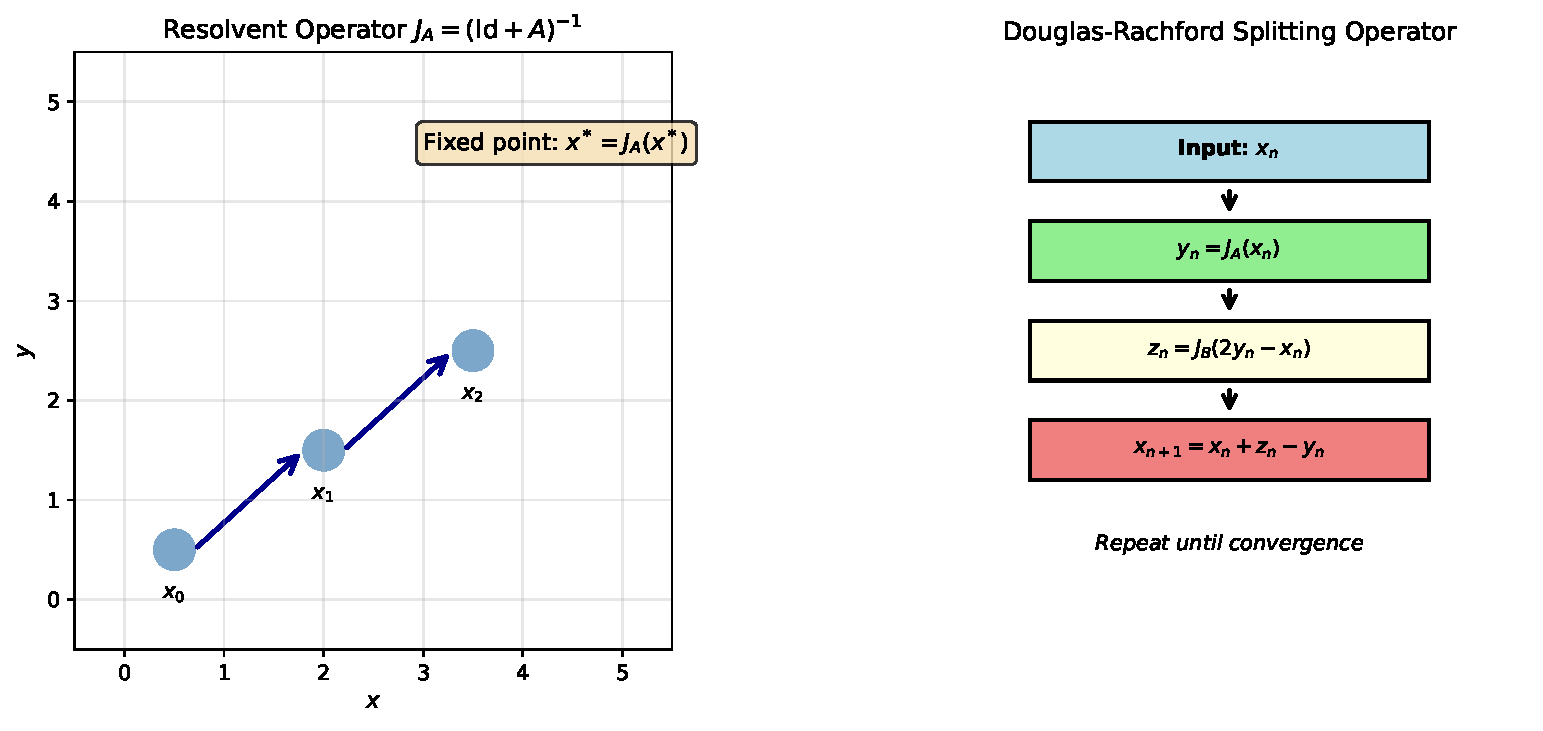
\includegraphics[width=0.95\textwidth]{resolvent_operator.pdf}
\end{center}

\end{frame}

% ============================================================================
% SECTION 5: VARIATIONAL INEQUALITIES
% ============================================================================

\section{Variational Inequalities}

\begin{frame}{Variational Inequality Problem}

\textbf{Definition:} Given $C \subseteq \mathcal{H}$ convex and $B: \mathcal{H} \to 2^{\mathcal{H}}$, the \textbf{variational inequality} is:
\[ \text{find } x \in C \text{ such that } (\forall y \in C) \quad \langle x - y \mid Bx \rangle \leq 0 \]

\vspace{0.3cm}
\textbf{Equivalence to monotone inclusions:}

Let $A = N_C$ (normal cone). Then:
\[ x \text{ solves VI} \Leftrightarrow 0 \in Ax + Bx \Leftrightarrow 0 \in N_C(x) + Bx \]

\vspace{0.3cm}
\textbf{Splitting approach:} Apply Douglas-Rachford or forward-backward to the equivalent inclusion.

\vspace{0.3cm}
\textbf{Projection method:}
\[ x_{n+1} = P_C(x_n - \gamma B x_n) \]

where $P_C$ is the projection operator onto $C$.

\end{frame}

\begin{frame}{Forward-Backward for Variational Inequalities}

\textbf{Proposition 26.25 (Forward-Backward Algorithm):} Let $f \in \Gamma_0(\mathcal{H})$, $\beta \in \mathbb{R}_{++}$, $B: \mathcal{H} \to \mathcal{H}$ be $\beta$-cocoercive, $\gamma \in ]0, 2\beta[$. Suppose:
\[ \text{find } x \in \mathcal{H} \text{ such that } (\forall y \in \mathcal{H}) \quad \langle x - y \mid Bx \rangle + f(x) < f(y) \]

has at least one solution. Given $x_0 \in \mathcal{H}$ and $(\lambda_n) \subseteq [0, \delta]$ with $\sum_n \lambda_n(\delta - \lambda_n) = +\infty$:

\begin{align*}
  y_n &= x_n - \gamma B x_n \\
  x_{n+1} &= x_n + \lambda_n(\text{prox}_f(y_n) - x_n)
\end{align*}

\textbf{Then:} $(x_n)$ converges weakly to a solution, and if $f$ or $B$ is strictly convex, convergence is strong.

\end{frame}

\begin{frame}[fragile]{Variational Inequality Example}

\textbf{Example:} Constraint qualification with quadratic penalty

\vspace{0.2cm}
\lstset{basicstyle=\ttfamily\footnotesize}
\begin{lstlisting}
import numpy as np

# Problem: min 0.5 ||Ax - b||^2 s.t. x in C = [0, 1]^n
# Equivalent VI: find x in C such that
#                 <x-y, A^T(Ax-b)> <= 0 for all y in C

def projection_simplex(x, s=1.0):
    """Project onto simplex: C = {x : sum(x)=s, x>=0}"""
    n = len(x)
    rho = np.sum(np.sort(x)[::-1]) - s
    idx = np.arange(n) + 1
    mask = np.sort(x)[::-1] - rho / idx > 0
    theta = (np.sum(np.sort(x)[::-1][mask]) - s) / np.sum(mask)
    return np.maximum(x - theta, 0)

def forward_backward_vi(A, b, x0, gamma=0.1, n_iter=100):
    """Solve min ||Ax-b||^2 s.t. x in simplex"""
    x = x0.copy()
    for n in range(n_iter):
        # Gradient of ||Ax-b||^2
        grad_f = A.T @ (A @ x - b)
        # Forward step
        y = x - gamma * grad_f
        # Backward step (projection)
        x = projection_simplex(y)
    return x

# Test problem
n, m = 10, 5
A = np.random.randn(m, n)
b = np.random.randn(m)
x0 = np.ones(n) / n
x_sol = forward_backward_vi(A, b, x0)
print(f"Solution norm: {np.linalg.norm(x_sol):.4f}")
\end{lstlisting}

\end{frame}

\begin{frame}{Monotone Inclusion Applications}

\begin{center}
  
\includegraphics[width=0.95\textwidth]{monotone_operators.pdf}
\end{center}

\end{frame}

% ============================================================================
% SECTION 6: CONVERGENCE AND NUMERICAL RESULTS
% ============================================================================

\section{Convergence and Numerical Analysis}

\begin{frame}{Convergence Rates}

\begin{center}
  
\includegraphics[width=0.95\textwidth]{convergence_behavior.pdf}
\end{center}

\vspace{-0.3cm}
\textbf{Key observations:}
\begin{itemize}
  \item \textbf{Linear convergence:} Achieved under strong monotonicity + cocoercivity
  \item \textbf{Superlinear convergence:} Possible with acceleration or additional structure
  \item \textbf{Residual vs distance:} Monotonic decrease in both error and residual
\end{itemize}

\end{frame}

\begin{frame}{Numerical Example: Proximal Point Algorithm}

\begin{center}
  
\includegraphics[width=0.95\textwidth]{numerical_example.pdf}
\end{center}

\vspace{-0.3cm}
\textbf{Trajectory analysis:}
\begin{itemize}
  \item \textbf{(top-left):} Convergence path in 2D space
  \item \textbf{(top-right):} Log-scale error decay (linear convergence)
  \item \textbf{(bottom-left):} Exponentially decreasing step sizes
  \item \textbf{(bottom-right):} Objective value monotonically decreasing to optimum
\end{itemize}

\end{frame}

\begin{frame}{Fixed Point Theory Summary}

\begin{center}
  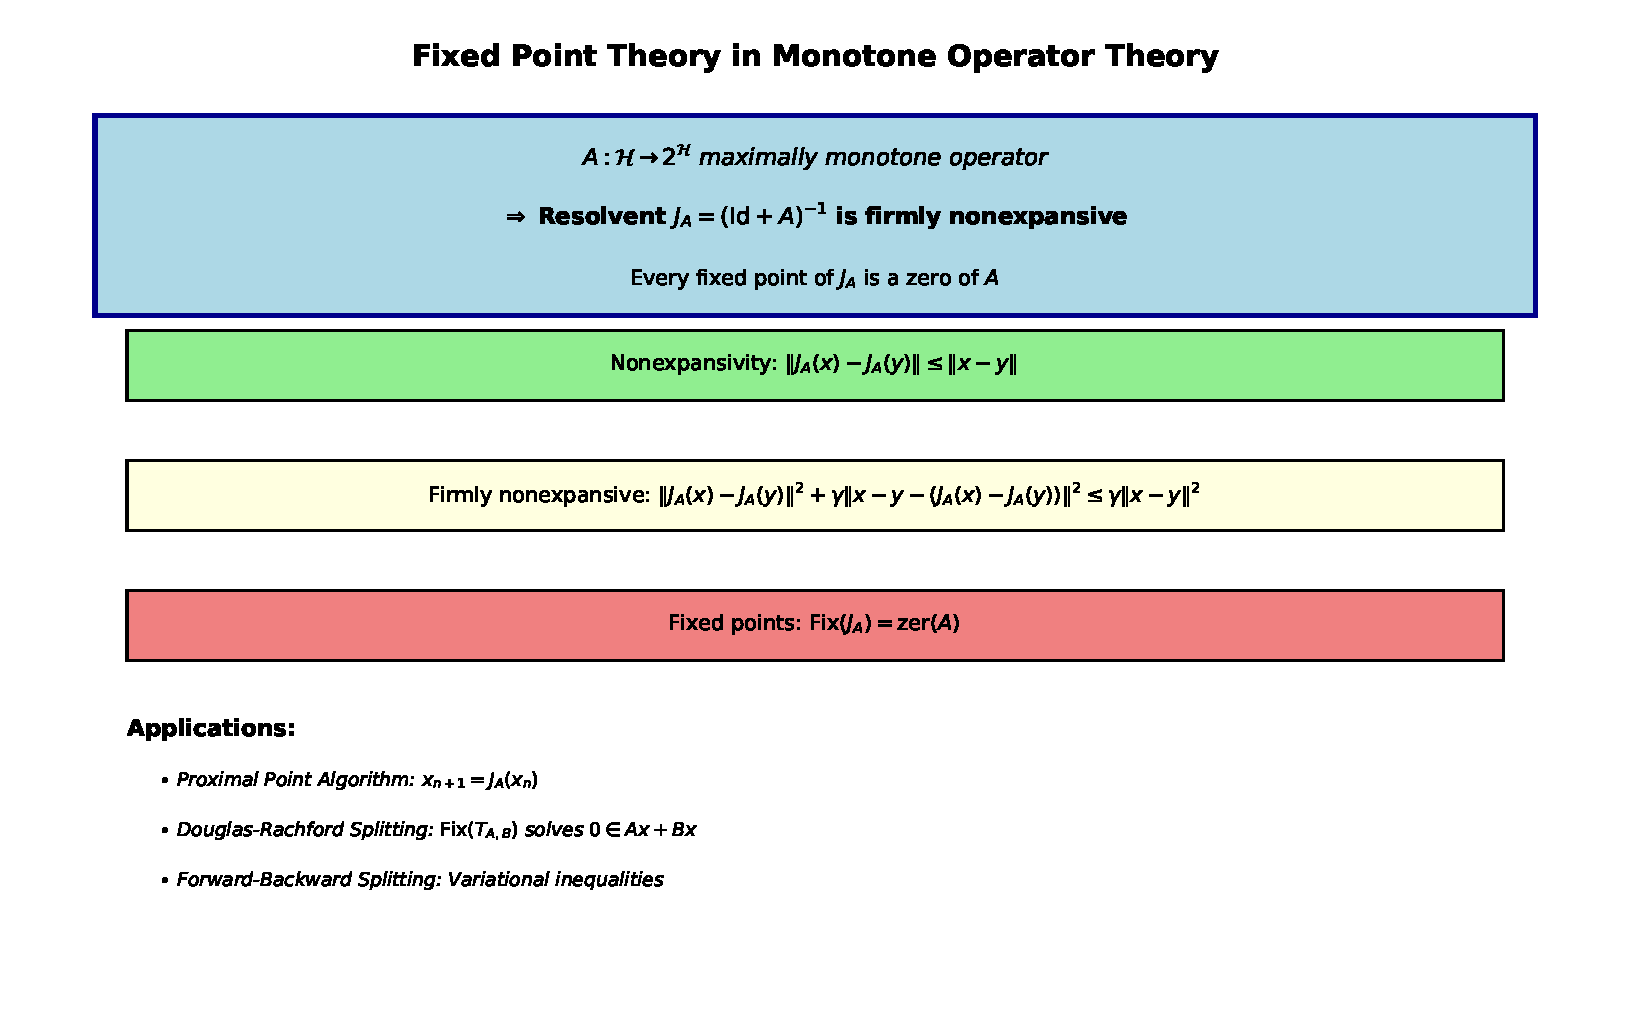
\includegraphics[width=0.95\textwidth]{fixed_point_theory.pdf}
\end{center}

\end{frame}

% ============================================================================
% SECTION 7: ADVANCED TOPICS
% ============================================================================

\section{Advanced Topics}

\begin{frame}[allowframebreaks]{Constrained Composite Inclusions}

\textbf{Problem 26.35:} General multiple operator composite inclusion.

Let $z \in \mathcal{H}$, $A: \mathcal{H} \to 2^{\mathcal{H}}$ be maximally monotone, $I$ a nonempty finite index set. For each $i \in I$:
\begin{itemize}
  \item $K_i$ is a real Hilbert space
  \item $r_i \in K_i$, $B_i: K_i \to 2^{K_i}$ maximally monotone
  \item $L_i \in \mathcal{B}(\mathcal{H}, K_i) \setminus \{0\}$
\end{itemize}

Solve the \textbf{primal inclusion}:
\[ \text{find } x \in \mathcal{H} \text{ such that } z \in Ax + \sum_{i \in I} L_i^*(B_i(L_i x - r_i)) \]

and the \textbf{dual inclusion}:
\[ \text{find } (v_i)_{i \in I} \in \bigoplus_{i \in I} K_i \text{ such that } (\forall i \in I) \quad -r_i \in L_i A^{-1}\left(z - \sum_{j \in I} L_j^* v_j\right) + B_i^{-1} v_i \]

\vspace{0.3cm}
\textbf{Solution:} Use Spingarn's method or modified Douglas-Rachford on product spaces.

\pagebreak

\textbf{Corollary 26.36:} Under suitable qualification conditions:
\[ z \in \text{ran}\left(A + \sum_{i \in I} L_i^* \circ B_i \circ (L_i \cdot -r_i)\right) \]

An iterative algorithm (Corollary 26.36):

\begin{align*}
  y_{1,n} &= x_n - \gamma \sum_{i \in I} L_i^* v_{i,n} \\
  p_{1,n} &= J_A(y_{1,n} + \gamma z) \\
  \text{(for each } i \in I \text{):} \\
  y_{2,i,n} &= v_{i,n} + \gamma L_i x_n \\
  p_{2,i,n} &= y_{2,i,n} - \gamma(r_i + J_{-\gamma B_i}(\gamma^{-1} y_{2,i,n} - r_i)) \\
  q_{2,i,n} &= p_{2,i,n} + \gamma L_i p_{1,n} \\
  v_{i,n+1} &= v_{i,n} - y_{2,i,n} + q_{2,i,n} \\
  q_{1,n} &= p_{1,n} - \gamma \sum_{j \in I} L_j^* p_{2,j,n} \\
  x_{n+1} &= x_n - y_{1,n} + q_{1,n}
\end{align*}

\end{frame}

\begin{frame}{Key Theoretical Results Summary}

\textbf{Main Theorems in Chapter 26:}

\begin{center}
  \begin{tabular}{p{3cm}|p{6cm}}
    \hline
    \textbf{Theorem} & \textbf{Result} \\
    \hline
    26.1 & Duality characterizations of zeros of $A + B$ \\
    \hline
    26.5 & Zeros of finite sums: $x = x_1 = \cdots = x_m$ \\
    \hline
    26.9 & Spingarn's partial inversion method converges \\
    \hline
    26.10 & Douglas-Rachford splitting convergence \\
    \hline
    26.11 & Proximal point algorithm weak convergence \\
    \hline
    26.16 & Linear convergence under strong monotonicity \\
    \hline
    26.20 & Forward-backward algorithm convergence \\
    \hline
    26.25 & Forward-backward for variational inequalities \\
    \hline
  \end{tabular}
\end{center}

\end{frame}

\begin{frame}{Connections to Other Chapters}

\textbf{Key references used:}
\begin{itemize}
  \item \textbf{Chapter 4:} Firmly nonexpansive operators and averaged operators
  \item \textbf{Chapter 15:} Duality, Fenchel conjugate, and dual problems
  \item \textbf{Chapter 16:} Properties of operators (cocoercivity, strong monotonicity)
  \item \textbf{Chapter 20:} Constrained optimization methods
  \item \textbf{Chapter 22-23:} Subdifferentials and proximal operators
  \item \textbf{Chapter 24:} Proximal point algorithms and special methods
\end{itemize}

\vspace{0.3cm}
\textbf{Forward references:}
\begin{itemize}
  \item Applications to variational inequalities (Section 26.7)
  \item Stochastic algorithms (extensions of deterministic framework)
\end{itemize}

\end{frame}

% ============================================================================
% CONCLUDING SLIDE
% ============================================================================

\begin{frame}{Chapter 26: Summary}

\textbf{Key Concepts:}
\begin{enumerate}
  \item \textbf{Resolvents:} $J_A = (\text{Id} + A)^{-1}$ map zeros of $A$ to fixed points of $J_A$

  \item \textbf{Splitting methods:} Douglas-Rachford and forward-backward decompose difficult problems

  \item \textbf{Fixed point iteration:} Proximal point algorithm converges weakly to zeros

  \item \textbf{Duality:} Solutions to $0 \in Ax + Bx$ and dual problem are characterized together

  \item \textbf{Convergence rates:} Linear under strong monotonicity, can be superlinear with acceleration
\end{enumerate}

\vspace{0.4cm}
\textbf{Main Applications:}
\begin{itemize}
  \item Variational inequalities on convex sets
  \item Composite optimization ($\min f + g$)
  \item Constrained monotone inclusion problems
  \item Operator splitting for parallel computation
\end{itemize}

\vspace{0.4cm}
\textbf{Practical Implementation:}
\begin{itemize}
  \item Choose algorithm based on operator structure
  \item Tune stepsizes $\gamma$ for convergence rate
  \item Use fixed point iteration for simplicity, splitting for modularity
\end{itemize}

\end{frame}

\end{document}
